\subsection{Vom Bild zum Vektor}
Der erste Schritt besteht darin, Bilder als Vektoren aufzufassen.
Das hat zwei Gründe: Erstens können wir diese nur so geeignet in Python darstellen und manipulieren.
Zweitens erlaubt uns das, Bilder in den Kontext der linearen Algebra zu bringen um deren mächtige Methoden anzuwenden.
Als Beispiel betrachten wir ein Bild der Auflösung $N=144$ Pixel (Breite) mal $M=180$ Pixel (Höhe), wie in Abbildung~\ref{fig:image_to_vector}.
Jedem Pixel wird nun eine reelle Zahl zwischen Null und Eins zugeordnet.
Nehmen wir das Pixel an der Stelle $\left(i,j\right)\in\mathbb N^M\times\mathbb N^N$.
Zum Beispiel entspricht $\left(1,N\right)$ dem Pixel in der oberen rechten Ecke des Bildes.
Diesem Pixel wird also eine Zahl $p_{ij}\in\left[0,1\right]$ zugeordnet.
Dabei bedeutet $p_{ij}=0$, dass das Pixel schwarz ist und $p_{ij}=1$, dass es weiss ist.
Die Zahlen dazwischen entsprechen den Graustufen.
Das gibt uns eine $N\times M$-Matrix deren Einträge gerade die $p_{ij}$ sind.
So können wir also ein schwarz-weiss Bild als Matrix auffassen.
Nun schreiben wir die Spalten dieser Matrix in einen Vektor wie in Abbildung~\ref{fig:image_to_vector} gezeigt.
Mit dieser Abbildungsvorschrift können wir jedem schwarz-weiss Bild der Auflösung $N\times M$ auf eindeutige Weise einen Vektor in $\left[0,1\right]^{N\cdot M}$ zuordnen.
Jeder solche Vektor lässt sich auch wieder als Bild darstellen.
Für diesen Schritt ist es egal ob das Bild ein Gesicht zeigt oder etwas anderes.
\begin{figure}[ht]
	\centering
	\begin{tabular}{m{3.5cm} m{1cm} c m{1cm} c}
		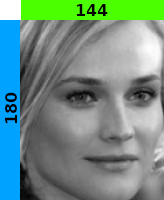
\includegraphics[width=0.2\textwidth]{images/vectormatrix/ImageToVector} &
		$\longrightarrow$ &
		$\begin{pmatrix}
			\textcolor{violet}{p_{11}} & \textcolor{orange}{p_{12}} & \cdots & \textcolor{olive}{p_{1N}} \\
			\textcolor{violet}{\vdots} & \textcolor{orange}{\vdots} & \ddots & \textcolor{olive}{\vdots} \\
			\textcolor{violet}{p_{M1}} & \textcolor{orange}{p_{M2}} & \cdots &  \textcolor{olive}{p_{MN}} \\
		\end{pmatrix}$ &
		$\longrightarrow$ &
		$\begin{pmatrix}
			\textcolor{violet}{p_{11}} \\
			\textcolor{violet}{\vdots} \\
			\textcolor{violet}{p_{M1}} \\
			\textcolor{orange}{p_{12}} \\
			\textcolor{orange}{\vdots} \\
			\textcolor{orange}{p_{M2}} \\
			\vdots \\
			\textcolor{olive}{p_{1N}} \\
			\textcolor{olive}{\vdots} \\
			\textcolor{olive}{p_{MN}} \\
		\end{pmatrix}$
	\end{tabular}
	\caption{Ein schwarz-weiss Bild kann als Matrix oder Vektor aufgefasst werden.}
	\label{fig:image_to_vector}
\end{figure}
\pagebreak[4]
\begin{aufgabe}
	Man betrachte das schwarz-weiss Bild, welches durch folgende Matrix beschrieben ist.
	\begin{equation*}
		\begin{pmatrix}
			1 & \frac{1}{4} \\
			\frac{1}{2} & 0 \\
			0 & \frac{3}{4} \\
		\end{pmatrix}
	\end{equation*}
	\begin{enumerate}[label=(\alph*)]
		\item Welche Werte für $N$ und $M$ beschreiben die Auflösung dieses Bildes?
		\item Wie sieht der Vektor aus, der dieses Bild beschreibt?
		\item Welches der folgenden drei Bilder entspricht dieser Matrix?
		
		\definecolor{onefourth}{rgb}{0.25, 0.25, 0.25}
		\definecolor{onehalf}{rgb}{0.5, 0.5, 0.5}
		\definecolor{threefourth}{rgb}{0.75, 0.75, 0.75}
		
		\qquad\qquad
		
\begin{tikzpicture}
			\draw[step=1cm,white,very thin] (0,0) grid (2,3);
			\fill[white] (0,0) rectangle (1,1);
			\fill[onefourth] (1,0) rectangle (2,1);
			\fill[onehalf] (0,1) rectangle (1,2);
			\fill[white] (1,1) rectangle (2,2);
			\fill[black] (0,2) rectangle (1,3);
			\fill[threefourth] (1,2) rectangle (2,3);
		\end{tikzpicture}
		\qquad\qquad
		
\begin{tikzpicture}
			\draw[step=1cm,white,very thin] (0,0) grid (2,3);
			\fill[black] (0,0) rectangle (1,1);
			\fill[threefourth] (1,0) rectangle (2,1);
			\fill[onehalf] (0,1) rectangle (1,2);
			\fill[black] (1,1) rectangle (2,2);
			\fill[white] (0,2) rectangle (1,3);
			\fill[onefourth] (1,2) rectangle (2,3);
		\end{tikzpicture}
		\qquad\qquad
		
\begin{tikzpicture}
			\draw[step=1cm,white,very thin] (0,0) grid (2,3);
			\fill[black] (0,0) rectangle (1,1);
			\fill[onefourth] (1,0) rectangle (2,1);
			\fill[onehalf] (0,1) rectangle (1,2);
			\fill[black] (1,1) rectangle (2,2);
			\fill[white] (0,2) rectangle (1,3);
			\fill[threefourth] (1,2) rectangle (2,3);
		\end{tikzpicture}
	\end{enumerate}
\end{aufgabe}
\begin{losung*}
	Die Lösung der ersten beiden Teilaufgaben kann von Abbildung~\ref{fig:image_to_vector} abgelesen werden.
	Für die letzte Teilaufgabe erinnern wir uns, dass die Zahlen in $\left[0,1\right]$ fliessend den Graustufen von Schwarz (Null) bis Weiss (Eins) entsprechen.
	\begin{enumerate}[label=(\alph*)]
		\item Die Auflösung ist $N=3$ mal $M=2$ Pixel.
		\item Der Vektor ist gegeben durch
		\begin{equation*}
			\begin{pmatrix}
				1 \\
				\frac{1}{2} \\
				0 \\
				\frac{1}{4} \\
				0 \\
				\frac{3}{4} \\
			\end{pmatrix}.
		\end{equation*}
		\item Das mittlere Bild entspricht der Matrix.
	\end{enumerate}
\end{losung*}
In unserem Python Code ist die Funktion, welche eine $N\times M$ Matrix auf diese Weise in einen Vektor der Länge $N\cdot M$ überführt, bereits implementiert.
Sie befindet sich im File \texttt{eigenfaces.py} und heisst \texttt{matrix\_to\_vector}.
Wir betrachten diese nun etwas genauer, um die Manipulation von Matrizen und Vektoren in Python zu lernen.
\begin{lstlisting}[style=python]
import numpy as np

def matrix_to_vector(P, M, N):
	v = np.zeros(M * N)
	for i in range(M):
		for j in range(N):
			v[j + N * i] = P[i, j]
	return v
\end{lstlisting}
Das Argument \texttt{P} ist eine  \texttt{M} mal \texttt{N} Matrix und besteht aus den Einträgen $p_{ij}\in\left[0,1\right]$ wie oben.
Auf die Einträge von Vektoren und Matrizen kann über die eckigen Klammern $[$ und $]$ zugegriffen werden.
Wir brauchen aber auch die Umkehrung dieser Operation.
Das ist der Zweck folgender Übung.
\begin{aufgabe}
	Ergänzen Sie im File \texttt{eigenfaces.py} die Funktion \texttt{vector\_to\_matrix(v, M, N)}.
	Dabei ist \texttt{v} ein Vektor der Länge $\texttt{M}\cdot\texttt{N}$ wie oben.
	Die Funktion soll die zu \texttt{v} gehörende Matrix zurück geben.
	Sie können die ihre Lösung überprüfen indem Sie das Skript \texttt{vector\_to\_matrix\_test.py} laufen lassen.
\end{aufgabe}
\begin{losung*}
	Bei einer richtigen Lösung sollte das Skript \texttt{vector\_to\_matrix\_test.py} das Foto aus Abbildung~\ref{fig:image_to_vector} generieren.
	Die Lösung könnte zum Beispiel so aussehen:
\begin{lstlisting}[style=python]
import numpy as np

def vector_to_matrix(v, M, N):
	P = np.zeros(M, N)
	for i in range(M):
		for j in range(N):
			P[i, j] = v[j + N * i]
	return P
\end{lstlisting}
\end{losung*}